\documentclass[5p,authoryear,square]{elsarticle}
\makeatletter 
\def\ps@pprintTitle{%
 \let\@oddhead\@empty
 \let\@evenhead\@empty
 \let\@evenfoot\@oddfoot} % Supprimer le bas de page ELSEVIER
\makeatother
\usepackage[utf8]{inputenc} % En unicode
\usepackage[T1]{fontenc}
\usepackage[french]{babel}
\usepackage[babel=true]{csquotes} % permet de faire \enquote{a} (« a »)
\usepackage[fleqn]{amsmath} % pour certains signes mathématiques
\usepackage{amsthm} % Pour \begin{gather}
\usepackage{booktabs} % pour \toprule (un style de tableau)
\usepackage{multirow} % Pour colonnes multiples des tableaux
\usepackage{amssymb} % Pour \leqslant (<=, >=)
\usepackage{float}
\usepackage{subcaption}
\usepackage{xcolor}
% \definecolor{refcolor}{HTML}{0000FF}        % blue for refs
% \definecolor{citecolor}{HTML}{FF00FF}       % violet/magenta for citations
% \definecolor{footnotecolor}{HTML}{FF00FF}   % magenta for footnotes


%\bibliographystyle{elsarticle-num}
\bibliographystyle{elsarticle-harv}

\usepackage[bookmarks=true,colorlinks=true,linkcolor = red,citecolor=red,urlcolor=red]{hyperref}
\usepackage[french,nameinlink,noabbrev]{cleveref}


\begin{document}

\begin{frontmatter}

\title{\textbf{Modélisation de l'effet dynamique d'un échantillon granulaire lâche par Méthode des Élements Discrètes}}

%% Group authors per affiliation:
\author{Viet Anh QUACH, Gaël COMBE, Vincent RICHEFEU}
\address{Laboratoire 3SR, Université Grenoble Alpes}

% \author{Encadré par Sandra Ulrich Ngueveu}
% \address{LAAS-CNRS, Toulouse}

\begin{abstract}
% * <mael65@gmail.com> 2015-04-22T06:55:22.738Z:
%
%  Qu'est-ce qu'on écrit là ?
%
% ^ <mael65@gmail.com> 2015-04-25T13:28:43.626Z.
Cet article  étudie deux méthodes utilisées dans le cadre du transport humanitaire en cas de crise (désastre, épidémie...). Le \emph{Covering Tour Problem} se focalise sur l'équité de distribution des vivres, alors que le \emph{Capacitated Vehicle Routing Problem} se concentre sur l'urgence de la distribution. Nous proposons une nouvelle approche mélangeant ces deux approches pour former une solution à la fois équitable et rapide.
Ce article a été rédigé dans le cadre du TER\footnotemark{} 2014-2015.

\end{abstract}

\begin{keyword}
CCVRP \sep CTP \sep CTP-CCVRP \sep CTP-VRP \sep Logistique de crise humanitaire\end{keyword}

\end{frontmatter}

\footnotetext{Travail encadré de recherche. Il s'agit d'un travail de trois mois, par équipe de 4 à 5 étudiants, effectué durant le long du deuxième semestre de M1 informatique, à l'université Toulouse 3 — Paul Sabatier.}


%\linenumbers
\section{Introduction}\label{introduction}
La logistique humanitaire intervient afin d'assurer l'organisation matérielle d'une organisation humanitaire. Elle se distingue de la logistique classique par les contraintes humaines qu'elle impose. \citep{campbell_routing_2008} distingue deux de ces contraintes par leur importance dans le cas humanitaire : l'urgence, c'est à dire le besoin d'une distribution rapide en cas de crise, et l'équité de la distribution, c'est à dire la nécessité que tous les habitants aient accès à l'aide sans distinction d'éloignement.

Par ailleurs, il convient de distinguer trois phases de la logistique humanitaire. La première, dite \emph{phase de préparation}, consiste par exemple à conserver un stock permanent pour permettre une réponse rapide à l’urgence. La seconde, la \emph{phase de réponse à l'urgence}, a pour objectif  la mise à disposition de vivres aux habitants des zones sinistrées. Enfin, la dernière phase dite  \emph{phase de reconstruction} intervient dans le long terme. Elle tire notamment une grande part de son savoir-faire dans les valeurs du développement durable.

La seconde phase combine à la fois les critères d'urgence et d'équité. C'est précisément sur cette phase que notre travail se porte.

% * <mael65@gmail.com> 2015-04-17T13:16:10.325Z:
%
%  Il faut expliquer pourquoi on a introduit les 3 phases maintenant !
%
% ^ <mael65@gmail.com> 2015-04-21T20:06:36.028Z.

\section{État de l'art} \label{etat_art}
\subsection{Restriction du domaine d'étude}
De nombreux problèmes de logistique liés à la phase de réponse à l'urgence ont été étudiés dans la littérature. Nous avons choisi de nous restreindre à la catégorie des problèmes de transport (qui est une composante de la logistique) dans le cas statique (c'est à dire où la demande n'évolue pas dans le temps) et où la demande est déterministe (elle ne relève pas de processus stochastiques et est connue sans incertitude).

Seuls deux problèmes, à notre connaissance, appartiennent à cette catégorie : le \emph{Covering Tour Problem} (CTP, discuté en \cref{ctp}) — et ses variantes — et le \emph{Cumulative Capacitated Vehicle Routing Problem} (CCVRP, discuté en \cref{ccvrp}).

% A FAIRE : Éxpliquer pourquoi on a trvaillé sur CTP ET CCVRP
% A FAIRE : ne plus utiliser les mots "sommets atteignables", "sommets à couvrir" mais plutôt 
% habitants, points de distributon, vivres, camions, dépôt, distance (et non coût)

\subsection{Le \emph{Covering Tour Problem}} \label{ctp}

Le \emph{Covering Tour Problem} (CTP) est caractérisé par un ensemble d'habitants et un ensemble de points de distribution. Introduit par \cite{gendreau_covering_1997}, ce problème prend en compte le fait que tous les habitants ne peuvent être visités par un camion, mais que les habitants sont capables de se déplacer vers le point de distribution le plus proche. La distance maximale que peut parcourir un habitant est fixée — on appellera le rayon de couverture cette distance. Le schéma en \cref{ctp_un_camion} donne un exemple de solution à ce problème.

Ce problème respecte ainsi le principe d'équité dans l'accès à l'aide. L'objectif du CTP peut être séparé en deux étapes \citep{jozefowiez_bi-objective_2007}. D'abord un \emph{Set Covering Problem} (SCP), où on détermine un sous-ensemble minimal de points de distributions permettant la couverture de tous les habitants. Ensuite, un \emph{Travelling Salesman Problem} (TSP), où on détermine le circuit de distance minimale d'un unique camion à capacité illimitée à travers ce sous-ensemble de points de distribution.

L'article de \cite{gendreau_covering_1997} cite plusieurs exemples théoriques d'utilisation du CTP : il pourrait être utilisé pour localiser les endroits optimaux pour placer des boîtes de poste, ou construire une route pour les équipes de réapprovisionnement de biens dans des pays en développement, dans lesquels les services médicaux ne peuvent être délivrés qu’à un ensemble de villages, mais où tous les habitants sont capables de marcher jusqu'au centre médical le plus proche (l'équivalent du point de distribution dans notre article).

L’article de \cite{hodgson_covering_1998} implémente le CTP de \cite{gendreau_covering_1997}, et pour la première fois dans un cas réel : l’acheminement de biens vers des centres de réapprovisionnement du Suhum District au Ghana. Cette étude distingue deux saisons : la saison sèche et la saison des pluies. Durant la seconde saison, certains points de distribution accessibles durant la saison sèche deviennent inaccessibles par la route, il faut donc pouvoir établir un nouveau parcours pour distribuer un maximum d’habitants. Cet article s’intéresse à ce problème en étudiant les conséquences du choix du rayon de couverture des points de distribution.

L’article de \cite{naji-azimi_covering_2012} se concentre sur le choix du placement de points de distribution secondaires approvisionnés depuis un dépôt unique par une flotte de camions non homogène : tous les camions ne transportent pas la même charge et ne transportent pas tous les mêmes types d'aide. Comme dans le cas du CTP classique, ces points de distributions doivent être déterminés pour permettre à chaque habitant d'être suffisamment proche d'un point de distribution. Ce CTP à plusieurs véhicules avait déjà été proposé par \cite{hachicha_heuristics_2000} (\emph{multiple-vehicle CTP}, m-CTP), mais \cite{naji-azimi_covering_2012} introduit une nouvelle notion de division de la distribution : un habitant peut être desservi par deux points de distribution. % Aussi, l'article ne donne pas de points de distribution obligatoires : ils sont tous facultatifs, contrairement au CTP classique où certains points de distributions doivent être obligatoirement visités.

\subsection{Le \emph{Cumulative Capacitated Vehicle Routing Problem}} \label{ccvrp}

Dans son article, \cite{campbell_routing_2008} remet en question l'utilisation des algorithmes de transport classiques dans le cas humanitaire. Il est expliqué que les notions d'urgence et d'équité ne sont pas respectées : la minimisation de la distance ne convient pas à l'aide humanitaire. L'une des deux formulations présentées, le \emph{Minimum-Average VRP} (minavg-VRP), est une formulation équivalente du \emph{Cumulative Capacitated Vehicle Routing Problem} (CCVRP) défini plus tard par  \cite{ngueveu_effective_2010} : à partir de plusieurs camions de capacité homogène, on veut trouver des tournées pour livrer un ensemble d'habitants. Contrairement au CTP, tous les habitants doivent être atteignables. Et contrairement au \emph{Vehicule Routing Problem} (VRP), qui minimise la distance parcourue par les camions en autorisant plusieurs camions, le CCVRP utilise une fonction objectif qui minimise la somme des temps d'arrivée chez les habitants.

\cite{ngueveu_effective_2010} montre que le CCVRP  aura tendance à utiliser le plus de camions possible par souci de rapidité, contrairement au VRP qui aura tendance à utiliser le moins de camions possible par souci d'économie.

\section{Analyse de l'existant et proposition d'un nouveau modèle}
\subsection{Constat et proposition}
Comme le suggère \cite{campbell_routing_2008}, la minimisation des coûts lors du choix d’un itinéraire ne permet pas d’assurer des temps d’arrivée convenables lorsqu’il s’agit de distribution d’aide humanitaire, et le CCVRP (ou min-avg VRP) donne de bonnes solutions respectant le critère d'urgence mais sans prendre en compte l'impossibilité d'accéder à tous les habitants, et donc ne respectant pas le critère d'équité. Au contraire, le CTP règle cette impossibilité, mais en gardant une fonction objectif basée sur la minimisation de la distance parcourue : le critère d'équité est pris en compte mais celui d'urgence ne l'est pas. Ce comparatif est résumé en \cref{comparatif}.

Contrairement au CTP classique qui n'autorise qu'un seul véhicule, le CCVRP permet l'utilisation de plusieurs véhicules. Une variante du CTP, le \emph{Multi-Vehicle Covering Tour Problem} (m-CTP)  proposée par \cite{hachicha_heuristics_2000} et reprise dans \cite{naji-azimi_covering_2012} permet d'élargir le problème en disposant de plusieurs camions à capacité limitée.

%Dans notre étude, nous avons comparé les m-CTP \emph{CTP-VRP}, car nous avons gardé les notions de partage de la distribution proposé par \cite{naji-azimi_covering_2012}.

Nous proposons un modèle de CTP multi-véhicules qui où l'on remplace la minimisation de la distance parcourue (la composante VRP du CTP) par la minimisation de la somme des temps d'arrivée aux points de distribution. Nous appellerons ce modèle \emph{CTP-CCVRP}. Le modèle mathématique se trouve en \cref{modele_ctpccvrp}. Ce modèle permettrait par exemple de diffuser des médicaments liés à une épidémie à travers des points de distribution. Ainsi, les habitants auraient accès aux traitements le plus rapidement possible.

Pour comparer ce nouveau modèle, nous avons pris comme référence le modèle proposé par \cite{naji-azimi_covering_2012}. Bien que très proche du m-CTP, il ajoute le partage de la distribution entre véhicules. Nous appellerons CTP-VRP ; le modèle mathématique est en \cref{modele_ctpvrp}.

\begin{figure*}
\centering \begin{tabular}{p{2cm} p{8cm} p{6cm}} \toprule
& \multicolumn{1}{c}{CTP} & \multicolumn{1}{c}{CCVRP} \\ \midrule
Objectif & Minimisation des coûts & Minimisation des temps d'arrivée \\ \\
Contraintes & Le dernier point de distribution visité impose une discrimination dans l'aide apportée & Nécessite que tous les habitants soient atteignables  \\  \\ 
Avantages & Permet de prendre en compte des situations où tous les habitants ne sont pas atteignables, ou lorsqu'on ne souhaite visiter qu'un sous-ensemble de points de distribution ; permet de respecter le critère d'équité & Permet de fournir l'aide en respectant le critère d'urgence \\ \bottomrule
\end{tabular} \caption{Tableau comparatif CTP vs. CCVRP} \label{comparatif}
\end{figure*}

\subsection{Méthodes de résolution utilisées}
Le modèle du CTP-CCVRP ainsi que la référence CTP-VRP sont formulés en programmation linéaire en nombres entiers (PLNE) à partir du modèle de donné dans \cite{naji-azimi_covering_2012}. Les formulations PLNE sont disponibles en \cref{modele_ctpvrp} et \cref{modele_ctpccvrp}, et le modèle GLPK est disponible sur le dépôt GitHub : \url{https://github.com/aheba/ctp/}.

L'instance est identique pour tous les tests. Elle a été créée arbitrairement et reprend l'exemple donné de \cite{naji-azimi_covering_2012}. Chaque habitant est couvert par au moins deux points de distribution pour que la partie SCP du CTP ait du sens et qu'un choix soit possible dans le sous-ensemble de points de distribution.

Nous avons utilisé le solveur \emph{GLPK} sur un Macbook Air 11" de mi-2011 à 1.6 Ghz. S'agissant de PLNE et donc de méthode exacte, l'instance utilisée est suffisamment petite pour que le temps de calcul ne dépasse pas 60 minutes.

\subsubsection{Légende des figures}
Dans chaque figure, qu'il s'agisse du CTP-VRP ou du CTP-CCVRP, l'arc de retour n'est pas affiché pour alléger les figures. Mais l'arc de retour est bien compté dans le calcul de la distance parcourue. 
\begin{figure}[ht]
	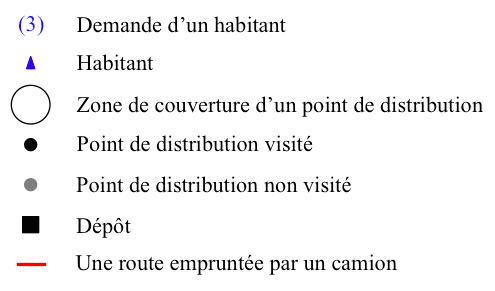
\includegraphics[width=2.5in]{figures/legende}
\end{figure}
\subsubsection{Explication des tables de résultat}
L'écart est calculé par la formule $(valeur_{CTP-VRP}-valeur_{CTP-CCVRP}) / valeur_{CTP-VRP}$. Si l'écart est positif, alors la valeur du CTP-CCVRP est plus grande que la valeur de référence (le CTP-VRP).
Les temps de transport (et donc les temps d'arrivée) sont arbitrairement calculés en utilisant les distances : on obtient des ordres de grandeurs identiques pour la distance parcourue et la somme des temps d'arrivée. Le temps d'arrivée maximal correspond au point de distribution atteint le dernier.
% * <mael65@gmail.com> 2015-04-17T15:49:28.216Z:
%
%  explication des colonnes du tableau
%
% ^ <mael65@gmail.com> 2015-04-22T14:12:53.533Z.

\subsection{Unique camion à capacité illimitée}
À partir du CTP-VRP, on peut revenir à une solution de CTP au sens de \citeauthor{gendreau_covering_1997} en limitant à un seul camion à capacité illimitée. Nous avons illustré cet exemple en \cref{ctp_un_camion}, que l'on peut comparer à la solution du CTP-CCVRP en \cref{ctpccvrp_un_camion}.

On obtient un écart de $-12.5\%$ (cf. \cref{table_un_camion}) concernant la somme des temps d'arrivée (cf. \cref{table_un_camion}), avec une faible augmentation de la distance de $+6.6\%$. En revanche, le dernier point de distribution desservi attend légèrement plus : c'est le seul exemple qui montre ce cas.

\subsection{Deux, trois et quatre camions}
Avec deux camions disponibles et une capacité de 18, on remarque que le CTP-CCVRP donne de biens meilleurs résultats que le CTP-VRP (\cref{ctpccvrp_deux_camions} et \cref{ctp_deux_camions}) en terme de temps d'arrivée (\cref{table_deux_camions}).

Le fait de passer à trois camions (\cref{ctpccvrp_trois_camions}) ne diminue la somme des temps d'arrivée que de $11\%$, tout en augmentant la distance parcourue de $20\%$ entre les deux solutions du CTP-CCVRP. Sans surprise, les résultats pour deux, trois et quatre camions sont les mêmes pour le CTP-VRP : celui-ci tend toujours à minimiser le nombre de camions, car son objectif est de minimiser la distance. 

Le passage de trois à quatre camions (\cref{ctpccvrp_quatre_camions}) confirme le phénomène : pour une toute petite diminution de la somme des temps d'arrivée, on en arrive à augmenter très fortement la distance parcourue (\cref{table_quatre_camions}).

\subsection{Conclusions}

Les solutions données par le modèle CTP-CCVRP peuvent être théoriquement intéressantes dans certains cas humanitaires. On remarque cependant que le fait d'ajouter un camion, à partir d'un certain nombre de camions, ne diminuera que peu la somme des temps d'attente, tout en augmentant très significativement la distance parcourue.

Pour que ce modèle puisse être utilisé, il serait d'abord nécessaire de trouver une méthode de résolution approchée (méta-heuristique par exemple) permettant de résoudre des instances de taille réelle. La formulation du problème étant différente de tous les problèmes déjà rencontrés dans la littérature, trouver une méta-heuristique n'est pas évident.

Le fait d'avoir les résultats d'instances réelles permettrait aux organisations humanitaires de savoir si, oui ou non, ces résultats sont cohérents avec la réalité logistique.

\section*{Annexes}
\begin{figure}[p] \centering
	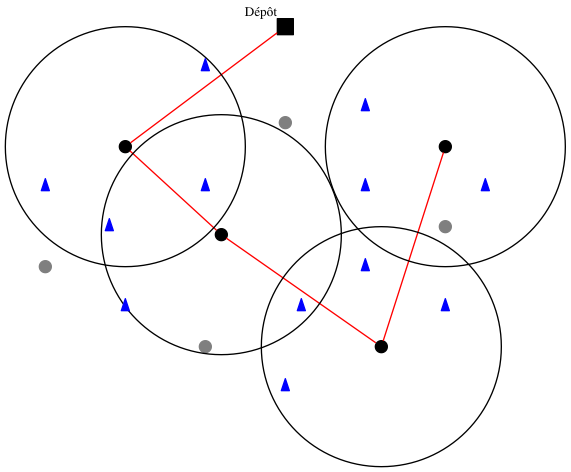
\includegraphics[width=3.4in]{figures/ctp_un_camion}
	\caption[]{Solution du CTP-VRP avec les contraintes du CTP classique. L'arc de retour n'est pas affiché mais fait bien partie du calcul de la fonction objectif.} \label{ctp_un_camion} 
\end{figure}

\begin{figure}[p]\centering
	\centerline{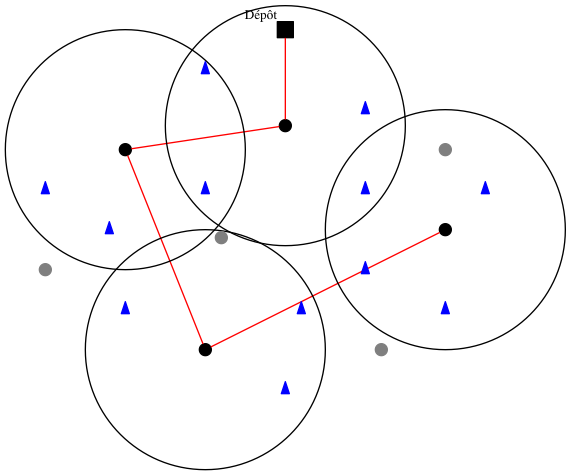
\includegraphics[width=3.4in]{figures/ctpccvrp_un_camion}}
	\caption[]{Solution du CTP-VRP avec un unique camion disponible et une capacité illimitée.} \label{ctpccvrp_un_camion}
\end{figure}

\begin{table}[p] \centering \begin{tabular}{@{\small}llll@{}} \toprule % utilise booktabs
 & {\footnotesize CTP-VRP} &  {\footnotesize CTP-CCVRP} & Écart \\ \midrule
Camions utilisés & 1 parmi 1 & 1 parmi 1 &  \\
Distance parcourue & 11.69 & 12.46 & +6.6\% \\
Somme temps d'arrivée & 22.39 & 19.59 & -12.5\% \\
Temps d'arrivée max. & 9.19 & 9.26 & +0.8\% \\ \bottomrule
\end{tabular} \caption{Comparatif CTP-VRP et CTP-CCVRP avec un unique camions et une capacité illimitée.} \label{table_un_camion}
\end{table}

\begin{figure}[p]\centering
	\centerline{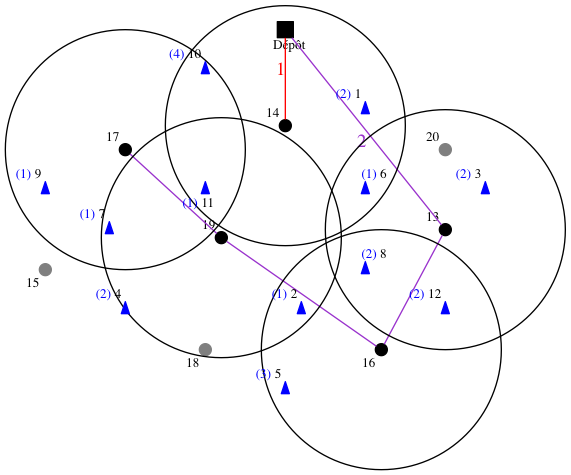
\includegraphics[width=3.4in]{figures/ctp_deux_camions}}
	\caption[]{Solution du CTP-VRP avec deux camions disponibles.} \label{ctp_deux_camions}
\end{figure}

\begin{figure}[p] \centering
	\centerline{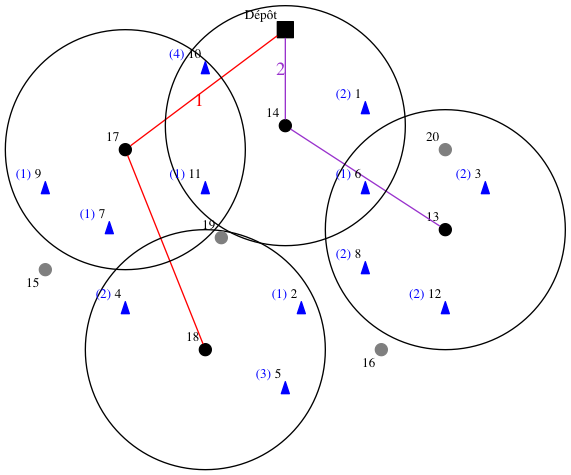
\includegraphics[width=3.4in]{figures/ctpccvrp_deux_camions}}
	\caption[]{Solution du CTP-CCVRP avec deux camions disponibles.} \label{ctpccvrp_deux_camions}
\end{figure}

\begin{table}[p] \centering \begin{tabular}{@{\small}llll@{}} \toprule % utilise booktabs
 & {\footnotesize CTP-VRP} &  {\footnotesize CTP-CCVRP} & Écart \\ \midrule
Camions utilisés & 2 parmi 2 & 2 parmi 2 &  \\
Distance parcourue & 13.87 & 16.1 & +16.1\% \\
Somme temps d'arrivée & 25.61 & 12.48 & -51.3\% \\
Temps d'arrivée max. & 8.97 & 5.19 & -42.1\% \\ \bottomrule
\end{tabular} \caption{Comparatif CTP-VRP et CTP-CCVRP avec deux camions disponibles et une capacité de 18.} \label{table_deux_camions}
\end{table}


\begin{figure}[p] \centering
	\centerline{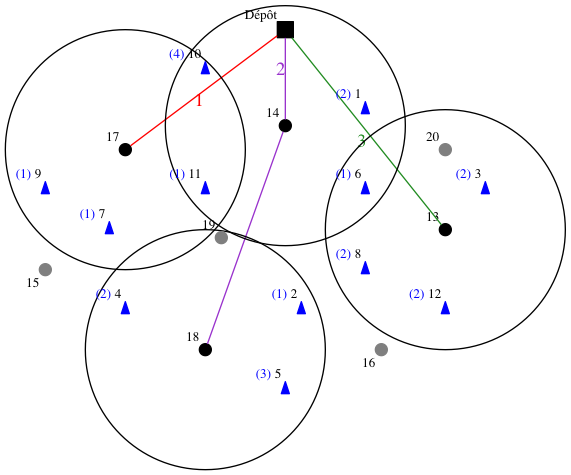
\includegraphics[width=3.4in]{figures/ctpccvrp_trois_camions}}
	\caption[]{Solution du CTP-CCVRP avec trois camions disponibles. Le résultat du CTP-VRP étant le même pour deux, trois et quatre camions, on se référera à \cref{ctp_deux_camions}.} \label{ctpccvrp_trois_camions}
\end{figure}


\begin{table}[p] \centering \begin{tabular}{@{\small}llll@{}} \toprule % utilise booktabs
 & {\footnotesize CTP-VRP} &  {\footnotesize CTP-CCVRP} & Écart \\ \midrule
Camions utilisés & 2 parmi 3 & 3 parmi 3 &  \\
Distance parcourue & 13.87 & 19.69 & +42.0\% \\
Somme temps d'arrivée & 25.61 & 11.07 & -56.8\% \\
Temps d'arrivée max. & 8.97 & 4.17 & -53.5\% \\ \bottomrule
\end{tabular} \caption{Comparatif CTP-VRP et CTP-CCVRP avec trois camions disponibles et une capacité de 18.} \label{table_trois_camions}
\end{table}


\begin{figure}[p] \centering
	\centerline{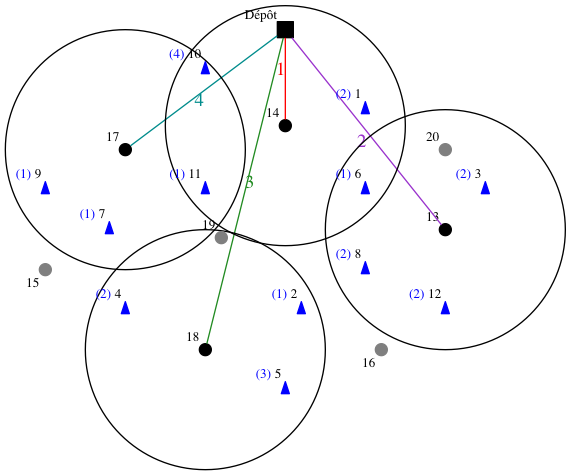
\includegraphics[width=3.4in]{figures/ctpccvrp_quatre_camions}}
	\caption[]{Solution du CTP-CCVRP avec quatre camions disponibles. Le résultat du CTP-VRP étant le même pour deux, trois et quatre camions, on se référera à \cref{ctp_deux_camions}.} \label{ctpccvrp_trois_camions} \label{ctpccvrp_quatre_camions}
\end{figure}

\begin{table}[p] \centering \begin{tabular}{@{\small}llll@{}} \toprule % utilise booktabs
 & {\footnotesize CTP-VRP} &  {\footnotesize CTP-CCVRP} & Écart \\ \midrule
Camions utilisés & 2 parmi 4 & 4 parmi 4 &  \\
Distance parcourue & 13.87 & 22.04 & +58.9\% \\
Somme temps d'arrivée & 25.61 & 11.02 & -57.0\% \\
Temps d'arrivée max. & 8.97 & 4.12 & -54.1\% \\ \bottomrule
\end{tabular} \caption{Comparatif CTP-VRP et CTP-CCVRP avec quatre camions disponibles et une capacité de 18.} \label{table_quatre_camions}
\end{table}
%
%\subsection{Modèle mathématique du CTP}\label{modele_ctp}
%Explication des variables de décisions utilisées dans le modèle.
%\begin{equation}
%Minimize\sum_{i<j}c_{ij}x{ij} ,
%\end{equation}
%sujet aux contraintes:

%\newcommand{\card}[1]{\ensuremath{\left\|#1\right\|}}
%\begin{gather}
%\sum_{v_k\in S_l} y_k \geqslant 1 (v_l\in W),\\%separer E de l'équation et faire un beau Sl
%\sum_{i<k}x_{ik}+\sum_{j>k}x_{kj} = 2y_k (v_k\in V),\\
%\sum_{v_i\in S, v_j\in V\setminus S  \textbf{ or } v_j\in S, v_i\in V\setminus S} x_{ij} \geqslant 2y_t (S \subset V , 2 \leqslant \card{S}\leqslant n-2,\\ T\setminus S \not = \emptyset),\\%voir probleme compil ici en plus \Card{S} marche pas
%x_{ij} \in \left\{0,1\right\},\\
%y_k =1 (v_k \in T),\\
%y_k \in \left\{0,1\right\} (v_k \in V\setminus T).
%\end{gather}
%Résumé du modèle.
\subsection{Modèle mathématique du CTP-VRP}\label{modele_ctpvrp}

Nous nous sommes inspirés du problème discuté par \cite{naji-azimi_covering_2012} pour définir le modèle de référence CTP-VRP permettant d'évaluer les performances du CTP-CCVRP. Le CTP-VRP est défini par un graphe orienté complet $G=(V,A)$ dans lequel $V$ représente l'ensemble des sommets et $A$ l'ensemble des arcs. On définit $V=\left\{0\right\} \cup I \cup J \cup \{m+1\}$,  $0$ étant le dépôt de départ et $\{m+1\}$ le dépôt d'arrivée (il s'agit en réalité du même dépôt), $I= \left\{1,...,n\right\}$ l'ensemble des habitants et $J= \left\{n+1,...,n+1+m\right\}$  l'ensemble des points de distribution. On notera aussi $K= \left\{1,...,l\right\}$ l'ensemble des véhicules. Contrairement au CTP de \cite{gendreau_covering_1997}, on ne définit pas de points de distribution que l'on doit visiter obligatoirement : tous les points de distribution sont optionnels. Cependant, tous les habitants $I$ doivent être couverts. L'ensemble des arcs est défini par $A$= $\left\{(v_i,v_j):v_i,v_j\in V\right\}$, et la matrice de distance $c_{ij}$ est définie sur $A$. Une flotte de véhicules $L$ est disponible, $Q$ étant la capacité (homogène) de tous les véhicules $k \in K$. Enfin, $\alpha = \left\{\alpha_{ij} \ i \in I, j \in J\right\}$ est une matrice dans laquelle $\alpha_{ij}$ est vrai si l'habitant $i$ est couvert par $j$ avec une distance inférieure à $d$, et faux sinon. Nous définissons également les variables de décision suivantes :
\begin{itemize}
 \item $D_{ijk}$ est la quantité de demande de l'habitant $i$ fournie par le $k^{ième}$ véhicule lors de sa visite au point de distribution $j$ ;
 \item $x_{ijk}$ est vraie si $arc(i,j)$ est utilisé par le véhicule $k$, et faux sinon ;
 \item $y_{jk}$ est vraie si le point distribution $j$ est visité par le véhicule $k$ ;
 \item $u_{jk}$ est une variable de décision libre permettant à la fois de représenter le temps d'arrivée du véhicule $k$ au point de distribution $j$ et  d'éliminer les \emph{sub-tour}.
 \end{itemize}

Le modèle est formulé comme suit :

\begin{equation}\label{somme_distances}
Minimiser \sum_{i=0}^{m}\sum_{j=1}^{m+1}\sum_{k=1}^{l} c_{ij} x_{ijk}
\end{equation}
 sous les contraintes :
\begin{gather}
\sum_{i=0}^{m}x_{ijk} = y_{jk}\qquad \forall j\in \{0\} \cup J, k \in K \label{sommet_atteignable_a_un_arc_entrant}\\ 
\sum_{i=0}^{n+1+m}x_{jik} = y_{jk}\qquad \forall j\in J \cup \{m+1\}, k \in K \label{sommet_atteignable_a_un_arc_sortant}\\ 
\sum_{j=0}^{m}x_{0jk} = 1 \qquad \forall k \in K \label{tournee_commence_depot}\\ 
\sum_{j=1}^{n+1+m}x_{j0k} = 1 \qquad \forall k \in K \label{tournee_termine_depot}\\
\sum_{j=1}^{m}\sum_{k=1}^{l} \alpha_{ij}D_{ijk} \geqslant d_{i}\qquad \forall i\in I \label{demande_satisfaite}\\
\sum_{i=1}^{n}D_{ijk} \leqslant Q_{k}y_{jk}\qquad \forall k \in K, j\in J \label{distribution_sommet_atteignable}\\
\sum_{i=1}^{n}\sum_{j=1}^{m}D_{ijk} \leqslant Q_k\qquad \forall k \in K \label{capacite_vehicule}\\
u_{ik} + c_{ij} - (1 - x_{ijk})T \leqslant u{jk} \notag \\
\qquad \forall i \in \{0\} \cup J, j \in J \cup \{0,n+1+m\}, k \in K \label{sub_tour}\\
x_{ijk} \in\left\{0,1\right\} \notag \\
\qquad\forall i,j\in\{0\}\cup J \cup \{n+m+1\}, i \neq j, k \in K \\
y_{jk} \in\left\{0,1\right\} \forall j\in J, k \in K\\ 
u_{ik} \geqslant 0  \qquad\forall i\in J, k \in K\\ 
D_{ijk} \geqslant 0 \qquad\forall i\in I, j\in J, k \in K\\ 
\end{gather}
La fonction objectif \ref{somme_distances} minimise la distance totale parcourue par les camions. Les contraintes \ref{sommet_atteignable_a_un_arc_entrant} et \ref{sommet_atteignable_a_un_arc_sortant} assurent que, pour chaque point de distribution $j$ et pour chaque véhicule $k$, il y a à la fois autant d'arcs entrants que d'arcs sortants de $j$. Les contraintes \ref{tournee_commence_depot} et \ref{tournee_termine_depot} contraignent l'existence d'un seul arc sortant du dépôt et un seul arc entrant au dépôt pour chaque véhicule $k$. La contrainte \ref{demande_satisfaite} spécifie qu'un habitant $i$ peut être approvisionné par plusieurs point de distribution $j$ (\enquote{distribution mutualisée}). La contrainte \ref{distribution_sommet_atteignable} relie les variables de décision $D_{ijk}$ à l'utilisation de chaque véhicule $k$ pour une livraison au point de demande $j$. La contrainte \ref{capacite_vehicule} impose le respect de la capacité $Q$ pour chaque véhicule $k$. La contrainte \ref{sub_tour}, tirée de \cite{ngueveu_effective_2010}, permet à la fois l'élimination des \emph{sub-tours} et le calcul des temps d'arrivée des camions aux points de distribution. $T$ est une constante arbitrairement grande.

\subsection{Modèle mathématique du CTP-CCVRP} \label{modele_ctpccvrp}
Le modèle CTP-CCVRP que nous proposons à partir du modèle du CTP-VRP ne nécessite que de changer la fonction objectif \cref{somme_distances}. Au lieu d'une minimisation des distances, on minimise la somme des temps d'arrivée aux points de distribution, c'est à dire la somme des $u_{jk}$. Ainsi, voici la nouvelle fonction objectif :
\begin{equation} \label{somme_temps_arrivee}
Minimiser \sum_{j \in J, k \in L} u_{jk}
\end{equation}


\bibliography{bibliographie.bib}

\end{document}